\documentclass[runningheads]{llncs}

\usepackage[T1]{fontenc}
\usepackage[utf8]{inputenc}
\usepackage{graphicx}
\usepackage{listings}
\usepackage{xcolor}
\usepackage{booktabs}
\usepackage{hyperref}

\hypersetup{
    colorlinks=true,
    linkcolor=blue,
    filecolor=magenta,      
    urlcolor=cyan,
    pdftitle={Módulo 3: Modelado de una Planta de Bicicletas en SIMUL8},
    pdfpagemode=FullScreen,
}

% Comando para cambiar "Abstract" por "Resumen"
\renewcommand{\abstractname}{Resumen}

\begin{document}

\title{Módulo 3: Simulación y Optimización de una Planta Industrial de Bicicletas mediante SIMUL8}
\subtitle{Modelado de Eventos Discretos y Análisis Costo-Beneficio}

\author{Allamand Francisco \and
Mateo Notti Echave \and
Facundo Dip \and
Pedro Elizalde}

\authorrunning{F. Allamand et al.}

\institute{Universidad Nacional de Cuyo\\
Facultad de Ingeniería\\
\email{franallamand05@gmail.com}}

\maketitle

\begin{abstract}
Este informe presenta el diseño, modelado y análisis económico-operativo de una planta de fabricación y comercialización de bicicletas utilizando el software de simulación de eventos discretos SIMUL8. El objetivo principal radica en evaluar la viabilidad financiera y la eficiencia de los flujos de trabajo concurrentes dentro de la empresa: la rama de producción manufacturera y la rama logística de atención al cliente. A través de la parametrización de variables de tiempo de ciclo fijas y distribuciones estocásticas exponenciales, se determinó el comportamiento de los inventarios intermedios, cuellos de botella y la rentabilidad integral de la operación. Los resultados financieros, recolectados sobre un período de operación simulado de una semana (2400 minutos), demuestran un balance superavitario, validando la configuración de recursos implementada.

\keywords{SIMUL8 \and Simulación de Eventos Discretos \and Optimización Industrial \and Cadena de Suministro \and Balance Financiero.}
\end{abstract}

\section{Introducción}
El diseño de sistemas industriales modernos exige metodologías capaces de predecir el comportamiento dinámico de los procesos antes de su implementación física. Las herramientas de simulación de eventos discretos permiten representar sistemas complejos donde los cambios ocurren en momentos específicos del tiempo, facilitando la identificación de ineficiencias logísticas y operacionales.

En este módulo, se empleó la versión educativa de escritorio del software SIMUL8 para modelar de manera integral una fábrica de bicicletas. El aprendizaje abarcó el análisis de criterios de entrada (\textit{Routing In}), lógica de despacho (\textit{Routing Out}), asignación dinámica de personal (\textit{Resources}) y la evaluación de estados de resultados monetarios integrados (\textit{Income Statement}). 

Para garantizar la reproducibilidad académica de esta experiencia, el archivo fuente de la simulación original (\texttt{.s8}) ha sido cargado en el repositorio compartido del equipo y se encuentra disponible para su descarga y ejecución directa a través del siguiente enlace digital: \\
\centerline{\href{https://drive.google.com/file/d/1iTyWoyoCG0DxSOM37P7rbQEZHBQsWhyl/view?usp=sharing}{Descargar Archivo de Simulación SIMUL8 - Fábrica de Bicicletas}}

\section{Fundamentos del Entorno de Simulación SIMUL8}
SIMUL8 se fundamenta en la interacción de componentes básicos orientados a objetos que replican la dinámica de una cadena de valor. Las entidades (\textit{Work Items}) fluyen a través de la infraestructura del modelo de acuerdo con reglas probabilísticas o determinísticas. Los elementos clave utilizados en el desarrollo de esta industria se detallan a continuación:

\begin{itemize}
    \item \textbf{Start Centers / Entry Points:} Puntos de generación donde ingresan las materias primas o los clientes al sistema bajo una tasa de arribo específica.
    \item \textbf{Storage Bins / Queues:} Zonas de acumulación pasiva que albergan entidades en espera de ser procesadas, permitiendo medir los niveles de inventario en proceso (WIP).
    \item \textbf{Work Centers / Puestos de Trabajo:} Unidades operativas activas donde se consume tiempo para transformar, ensamblar o testear las entidades. Poseen eficiencias, capacidades y costos de uso asociados.
    \item \textbf{Exit Houses / End Points:} Puntos de salida que contabilizan el egreso de productos terminados, ventas exitosas o pérdidas del sistema.
    \item \textbf{Resources / Operarios:} Recursos humanos o mecánicos limitados requeridos por los puestos de trabajo para ejecutar sus operaciones.
\end{itemize}

\section{Evolución del Aprendizaje con SIMUL8}
El dominio de la herramienta se alcanzó mediante un proceso pedagógico incremental, transitando desde la abstracción lineal básica hacia la modelización de redes industriales complejas e interdependientes:

\begin{enumerate}
    \item \textbf{Modelado de Flujos Lineales Básicos:} La introducción al entorno consistió en representar el recorrido de alumnos que ingresan a la universidad hasta su posterior egreso. Este ejercicio inicial permitió comprender la mecánica elemental de los tiempos de ciclo, las colas de espera y la asignación básica de capacidades.
    \item \textbf{Integración de Parámetros Económicos:} Posteriormente, se expandió el alcance de los modelos lineales para dotarlos de utilidad en la toma de decisiones estratégicas. Para ello, se incorporaron variables financieras avanzadas, tales como costos de operación por minuto, costos de capital y amortizaciones de maquinaria, transformando una simulación puramente matemática en un cuadro de mando financiero integral.
    \item \textbf{Sistemas de Ramas Concurrentes y Logística de Pérdidas:} Finalmente, mediante el estudio analítico de industrias arquetípicas como el modelo básico de McDonald's, se aprendió a vincular y sincronizar dos ramas operativas de naturaleza disímil dentro de un mismo entorno: la rama de producción manufacturera y la rama de atención al cliente. En esta etapa se dominó la introducción de factores de pérdidas estocásticas (descarte de producto, mermas logísticas y abandono de clientes por disconformidad), logrando un nivel de fidelidad representativa óptimo para el diseño de plantas reales.
\end{enumerate}

\section{Modelado de la Industria de Bicicletas}
El sistema desarrollado para la entrega final integra de manera síncrona la cadena productiva con la dinámica comercial de captación de demanda. El layout general implementado se visualiza en la Figura~\ref{fig:layout}.

\begin{figure}[htbp]
    \centering
    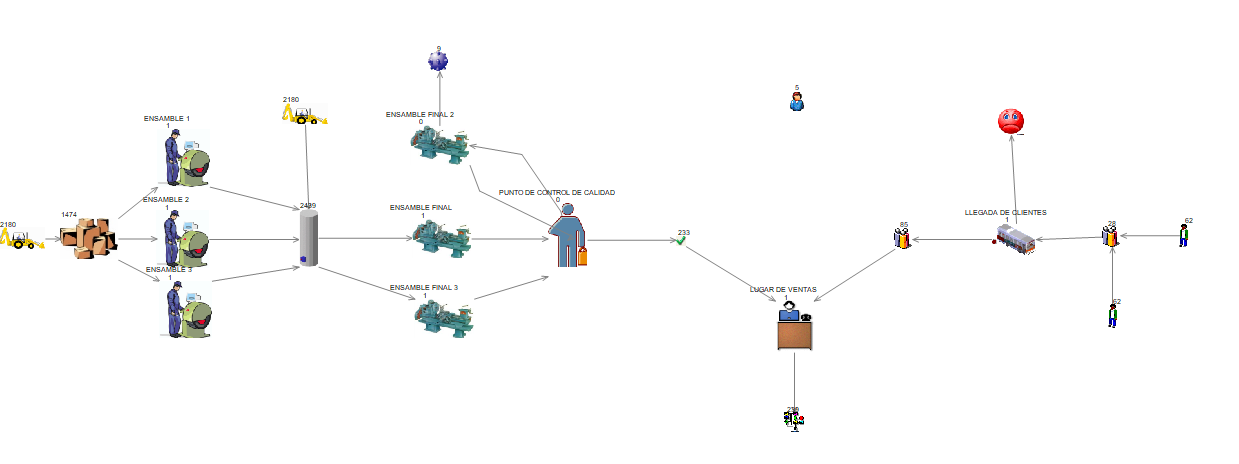
\includegraphics[width=\textwidth]{fotoindustria.png}
    \caption{Layout integral del sistema de manufactura y ventas en la interfaz de SIMUL8.}
    \label{fig:layout}
\end{figure}

\subsection{Estructura de la Rama Productiva (Flujo Izquierdo)}
La manufactura se divide en fases consecutivas de abastecimiento, pre-ensamble, ensamble final y control de calidad adaptativo:

\begin{enumerate}
    \item \textbf{Ingreso de Materia Prima:} Representa la llegada de los cuadros base de las bicicletas. Se configuró con una distribución constante (\textit{Fixed}) con un valor de 11 minutos y un costo directo de adquisición de \$200 por unidad. Estos se acumulan en el \textit{Depósito de Cuadros}.
    \item \textbf{Puestos de Pre-Ensamble concurrentes:} El depósito alimenta en paralelo a tres estaciones homogéneas denominadas \textit{Ensamble 1}, \textit{Ensamble 2} y \textit{Ensamble 3}. Cada puesto cuenta con restricciones estrictas de recursos (mínimo y máximo de 1 operario asignado), una eficiencia del 100\%, tiempo de procesamiento de distribución \textit{Fixed} de 10 minutos, un costo de capital de \$5000, costo de uso por minuto de \$0.30 y un costo variable de componentes añadidos de \$150 por unidad.
    \item \textbf{Almacenamiento Intermedio e Insumos:} Los subconjuntos convergen en una segunda etapa de almacenamiento tipo silo (\textit{Almacenamiento 2}), donde se simula mecánicamente la adición de componentes complementarios (ruedas, transmisiones y manubrios) requeridos para el armado definitivo.
    \item \textbf{Ensamble Final y Control de Calidad:} El flujo se ramifica hacia estaciones de \textit{Ensamble Final} operadas por un operario individual, con distribución \textit{Fixed} de 10 minutos, costo de capital de \$3000, costo de uso de \$0.25/min y \$50/unidad. Las bicicletas terminadas ingresan al \textit{Punto de Control de Calidad}, dotado de una célula flexible de inspección de entre 2 y 3 operarios simultáneos y un tiempo fijo de revisión de 2 minutos.
    \item \textbf{Lógica de Retrabajo Estocástico:} El ruteo de salida del puesto de control se parametrizó de forma porcentual para evaluar fallas:
    \begin{itemize}
        \item Un \textbf{95\%} de los productos aprobados se dirigen al \textit{Lugar de Ventas} (flujo conforme).
        \item Un \textbf{5\%} de productos defectuosos se desvían al puesto \textit{Ensamble Final 2} para su revisión. Esta estación secundaria (1 operario, tiempo \textit{Fixed} de 10 minutos) posee un comportamiento crítico: el 50\% de sus salidas se recuperan y regresan a la fila de control de calidad, mientras que el otro 50\% se descarta permanentemente debido a fallas estructurales insubsanables.
    \end{itemize}
\end{enumerate}

\subsection{Estructura de la Rama de Clientes (Flujo Derecho)}
Representa la llegada de la demanda al establecimiento mediante transporte corporativo:
\begin{itemize}
    \item \textbf{Fuentes de Demanda:} Se modelaron dos flujos de clientes independientes mediante distribuciones estocásticas exponenciales: \textit{Zona Centro} con una media de 35 minutos y \textit{Otras Zonas} con una media de 45 minutos.
    \item \textbf{Logística de Traslado:} Ambos grupos confluyen en un andén donde un micro de la empresa realiza traslados periódicos hacia el edificio comercial. El proceso de admisión de la \textit{Llegada de Clientes} posee un tiempo promedio (\textit{Average}) de 50 minutos.
    \item \textbf{Análisis de Tolerancia a la Espera:} Debido a las demoras del transporte, se configuró una regla de salida condicional en la fila de espera del edificio de ventas: el \textbf{90\%} de los clientes aguarda su turno, mientras que el \textbf{10\%} abandona las instalaciones frustrado por la demora. Cada abandono genera penalizaciones de \$1 en costo de capital debido al impacto negativo en el marketing de la empresa.
\end{itemize}

\subsection{Unión de Ramas: Punto de Venta Efectiva}
Las trayectorias de los clientes conformes y de las bicicletas aprobadas convergen de forma síncrona en el \textit{Lugar de Ventas}. Este nodo de acoplamiento es atendido por 2 operarios fijos y trabaja bajo una distribución de tiempo promedio (\textit{Average}) de 2 minutos. Cada transacción completada despacha una unidad hacia la salida de ventas efectivas, generando un ingreso bruto (\textit{Revenue}) de \$14000 por bicicleta comercializada.

\section{Análisis de Resultados Financieros y Operacionales}
La simulación fue ejecutada bajo parámetros rigurosos de tiempo de operación, configurados en las propiedades del reloj del sistema (\textit{Clock Properties}) detallados en la Tabla~\ref{tab:parametros}:

\begin{table}[h]
\centering
\caption{Parámetros de temporización de la corrida de simulación.}
\label{tab:parametros}
\begin{tabular}{ll}
\toprule
\textbf{Parámetro del Reloj} & \textbf{Valor Asignado} \\ \midrule
Unidades de Tiempo & Minutos \\
Formato de Hora & Tiempo y Día (Clock Face) \\
Días Laborales Semanales & 5 días \\
Tiempo de Jornada Diaria & 8 horas (08:00 a 16:00) \\
Período de Estabilización (\textit{Warm Up}) & 30 minutos \\
Período de Recolección de Datos & 2399.4999 minutos \\
\textbf{Tiempo Total de Simulación por Corrida} & \textbf{2400 minutos (1 Semana)} \\ \bottomrule
\end{tabular}
\end{table}

\subsection{Evaluación del Balance de Ingresos y Costos}
El modelo incorporó una plantilla de personal global de \textbf{12 empleados} con una tarifa corporativa fijada en \textbf{\$6000 la hora por operario}. Los costos operativos de mano de obra se integraron con los costos de capital y los costos variables de uso por unidad de los puestos de trabajo dentro de la herramienta financiera integrada de SIMUL8 (\textit{Finance Income Statement}). 

Al procesar la corrida bajo el período consolidado de una semana de actividad industrial, el sistema arrojó métricas estables con variaciones estadísticas mínimas entre réplicas:

\begin{itemize}
    \item \textbf{Costos Totales Operativos:} $\approx$ \$3,000,000 (derivados de sueldos de personal, costos de materia prima base, penalizaciones por pérdida de clientes y amortizaciones de maquinaria).
    \item \textbf{Ingresos Totales Brutos (Revenue):} $\approx$ \$3,300,000 (acumulados por la venta de bicicletas aptas a \$14,000 por unidad).
    \item \textbf{Utilidad Neta Semanal:} $\approx$ \textbf{+\$300,000}.
\end{itemize}

El resultado positivo confirma que la tasa de producción de las tres líneas de ensamble iniciales y las estaciones finales es capaz de absorber los costos fijos de la estructura de personal, logrando un equilibrio operativo sustentable. No obstante, el 10\% de pérdidas detectado en el transporte de clientes y el 2.5\% de descarte neto en el lazo de retrabajo representan áreas de oportunidad para futuras optimizaciones de capacidad.

\section{Conclusión}
La modelización de la planta industrial de bicicletas en SIMUL8 permitió afianzar conceptos prácticos de investigación operativa y gestión de la producción. A diferencia de los análisis de capacidad estáticos tradicionales, la simulación de eventos discretos expuso la interacción real entre variables determinísticas de manufactura y los arribos estocásticos de la demanda. 

Los balances arrojados por el \textit{Income Statement} validan que la configuración actual de 12 operarios y tres líneas de ensamble paralelas es económicamente viable bajo una semana tipo de 40 horas de labor. Esta metodología dota al ingeniero de herramientas críticas para justificar inversiones de capital, dimensionar inventarios de seguridad y mitigar riesgos financieros en entornos de manufactura complejos.

\end{document}